

\begin{figure}[t]
  \centering
  \begin{minipage}[b]{0.39\textwidth}
    \centering
    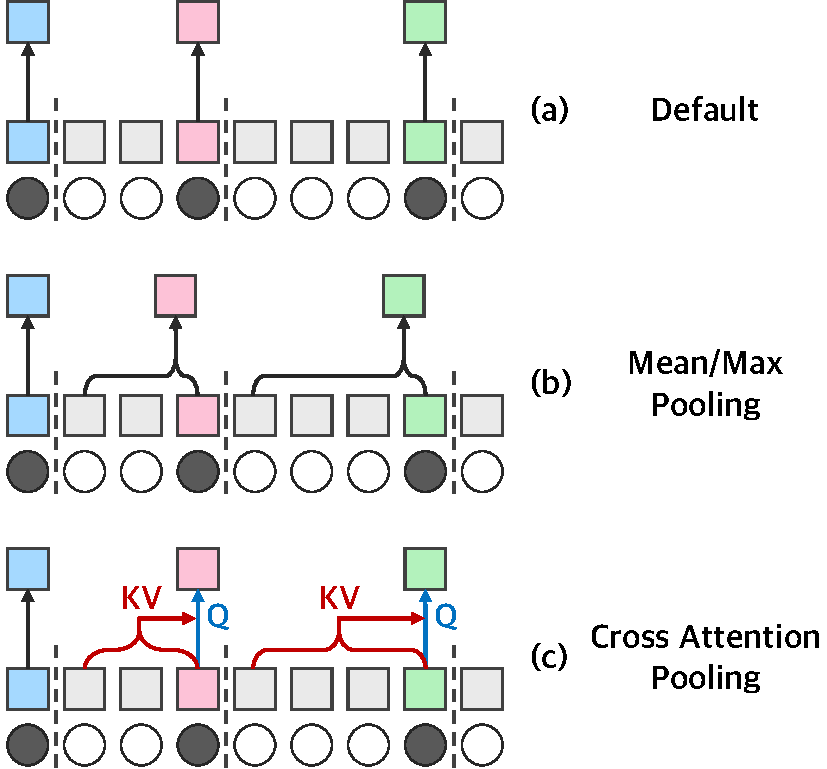
\includegraphics[width=\linewidth]{fig_img/pooling.pdf}
  \end{minipage}
  \hfill
  \begin{minipage}[b]{0.59\textwidth}
    \centering
    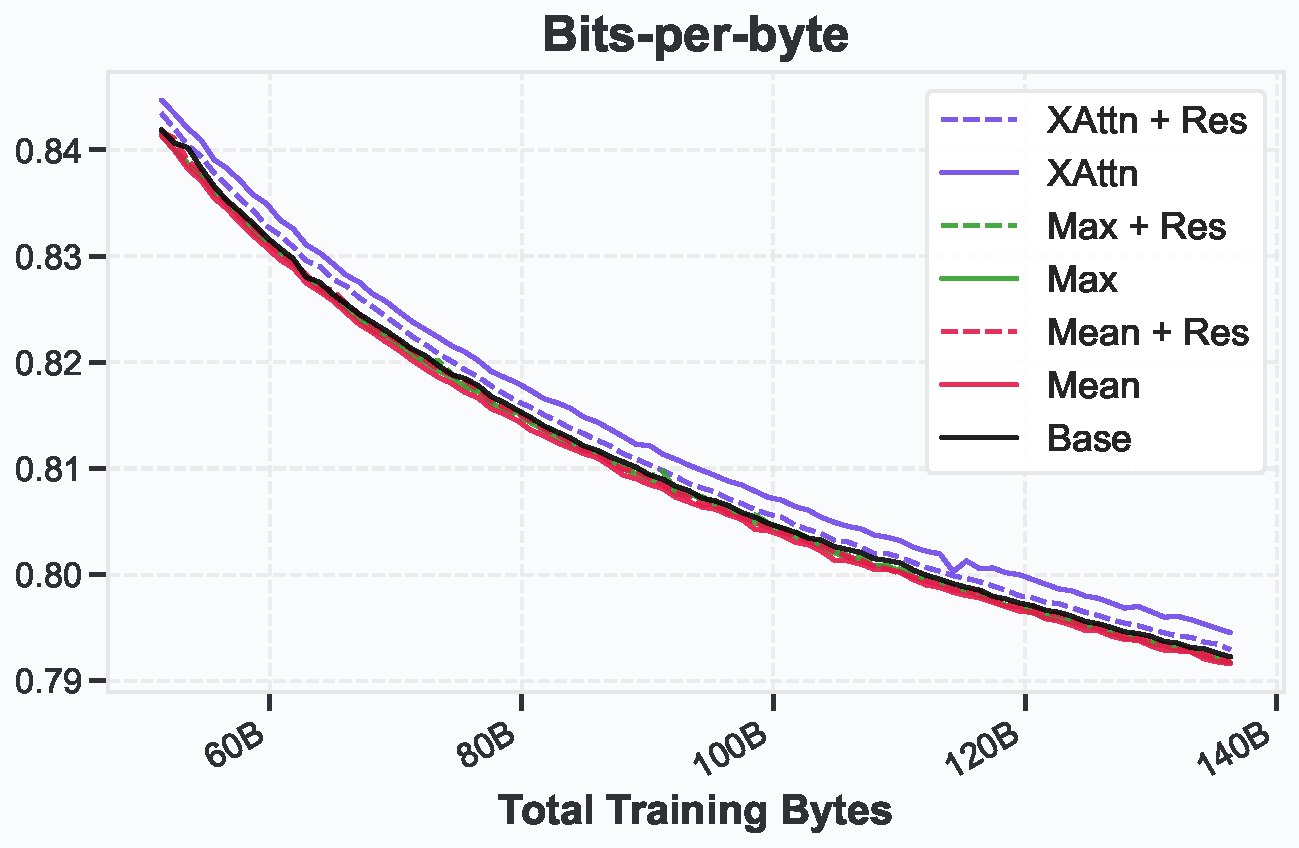
\includegraphics[width=\linewidth]{fig_img/abl_pool.pdf}
  \end{minipage}
  \caption{
    \textbf{Compression Methods in \chunk{}.} 
    Default: \model{}'s Downsample operation \textbf{(left-a)}.
    Max/Mean: Channel-wise max and mean pooling within boundaries \textbf{(left-b)}.
    XAttn: Cross-attention pooling within boundaries \textbf{(left-c)}.
    \texttt{+Res}: Adds boundary vector residuals to compressed outputs.
  }
  \label{fig: abl_pool}
\end{figure}
